\section{Analog-to-Digital Converter (ADC)}

\important{SEP Handouts: 05A\_ADC\_Beilage und 05B\_ADC\_DAC\_forStudents}

\begin{definition}{ADC Overview}\\
An Analog-to-Digital Converter (ADC) converts continuous analog signals into discrete digital values:
\begin{itemize}
    \item Transforms analog voltage levels into corresponding digital values
    \item Resolution determined by number of bits (N)
    \item $2^N$ possible digital values (e.g., 12-bit ADC has 4096 levels)
    \item Converts real-world continuous signals (temperature, pressure, etc.) into digital form for processing
\end{itemize}

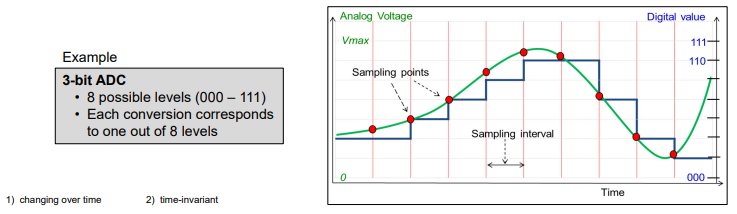
\includegraphics[width=0.8\linewidth]{adc_functionality.png}
\end{definition}

\begin{concept}{ADC Characteristics}\\
    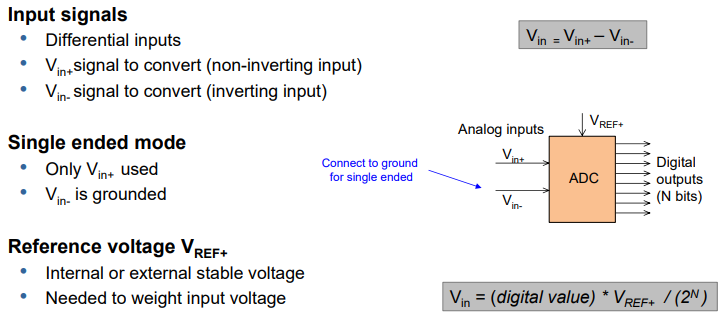
\includegraphics[width=0.7\linewidth]{adc_characteristics.png}
\end{concept}

\begin{theorem}{ADC Terminology}
Key terms and concepts:

\begin{minipage}{0.6\linewidth}
\begin{itemize}
    \item \textbf{Resolution}: Number of bits (N) in the digital output\\ (size of digital word)
    \item \textbf{LSB} (Least Significant Bit): Smallest detectable voltage change
    $$LSB = \frac{V_{REF}}{2^N}$$
    \item \textbf{FSR} (Full Scale Range): Range between minimum \\ and maximum digital codes
    $$FSR = V_{REF} - 1 LSB$$
    \item \textbf{Reference Voltage} ($V_{REF}$): Voltage that defines the ADC's full-scale range
\end{itemize}
\end{minipage}
\begin{minipage}{0.4\linewidth}
    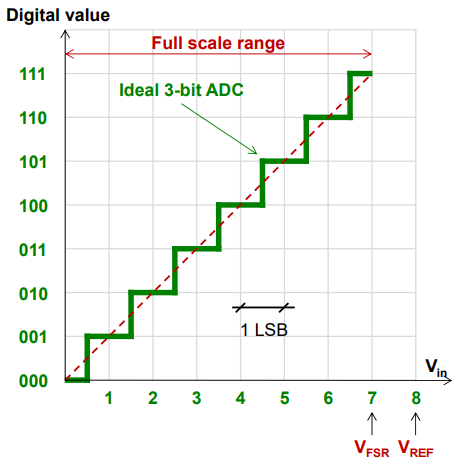
\includegraphics[width=0.9\linewidth]{adcconceptsandterminology.png}
\end{minipage}

\textbf{Sampling Rate}: Number of conversions per second
\begin{itemize}
    \item Input signal sampled at discrete points in time $\rightarrow$ discontinuities
    \item Should be at least twice the highest frequency component of input signal (Sampling theorem)
\end{itemize}
\textbf{Conversion Time}: Time from start of sampling to digital output availability
\begin{itemize}
    \item Programming a higher resolution may increase conversion time
\end{itemize}
\textbf{Monotonicity}: ADC output should not decrease with increasing input voltage
\begin{itemize}
    \item Increase of Vin results in increase or no change of digital output and vice-versa
\end{itemize}
\end{theorem}

\subsubsection{ADC Operation Principles}

\begin{concept}{Flash ADC (Parallel ADC)}
\begin{itemize}
    \item Uses comparators for each voltage level
    \item Input voltage compared to reference voltages simultaneously
    \item Fast but requires many components (e.g., 255 comparators for 8-bit)
    \item High power consumption and complexity (consumes large chip area)
    \item Network of $2^N$ resistors to divide $V_{REF}$ into $2^N$ levels
    \item $2^N - 1$ analog comparators for N-bit ADC 
    \item Compare input signal to divided reference voltages
    \item Encoder transforms digital comparator results into N-bit word
\end{itemize}
\end{concept}

\begin{theorem}{Example Flash ADC}\\
    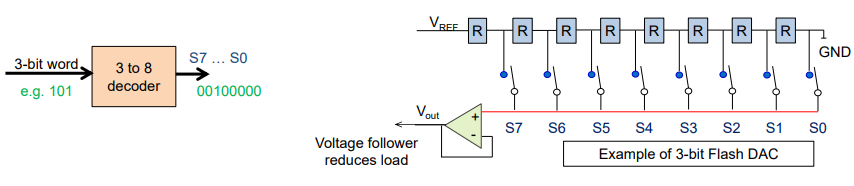
\includegraphics[width=\linewidth]{flashadc.png}
\end{theorem}

\begin{concept}{Successive Approximation Register (SAR) ADC}
\begin{itemize}
    \item Approach $V_{in}$ using successive division by 2 (binary search)
    \item Start with half the digital value (MSB=1, all other bits=0)
    \item DAC generates analog value $V_{D A C}$ that is compared to $V_{\text {in }}$
    \item If $\mathrm{V}_{\text {DAC }}<\mathrm{V}_{\text {in }} \rightarrow$ keep MSB at 1 , otherwise set MSB to 0
    \item Continue with other N bits in same way ( N steps)
\end{itemize}
Properties:
\begin{itemize}
    \item Compares input to successive approximations
    \item Takes N steps for N-bit resolution
    \item Good balance of speed, power, and complexity (up to 5 Msps, resolution from 8 to 16 bits)
    \item Most common in microcontrollers
\end{itemize}
\end{concept}

\begin{theorem}{Example SAR ADC}\\
    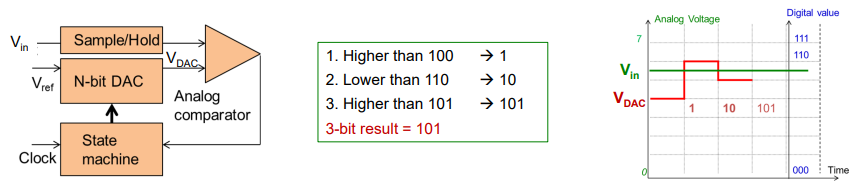
\includegraphics[width=\linewidth]{saradc.png}
\end{theorem}

\subsubsection{ADC Features (good to know but not really relevant)}
\begin{concept}{Analog Watchdog}
The Analog Watchdog monitors ADC conversion results against programmable thresholds:
\begin{itemize}
    \item Generates an interrupt if a conversion result is outside the threshold range
    \item Can be configured to monitor a single channel or all channels
    \item Useful for detecting abnormal voltage levels without CPU polling
    \item Programmable high and low thresholds
\end{itemize}
Applications:
\begin{itemize}
    \item Over-voltage/under-voltage detection
    \item Temperature limit monitoring
    \item Battery level monitoring
\end{itemize}
\end{concept}


\raggedcolumns
\columnbreak

\subsection{ADC Errors and Characteristics}

\begin{definition}{Sampling Theorem}
According to the Nyquist-Shannon sampling theorem:
\begin{itemize}
    \item Sampling rate must be at least twice the highest frequency component of the input signal
    \item $f_{sampling} \geq 2 \times f_{max}$
    \item Prevents aliasing (false lower frequencies appearing in sampled signal)
\end{itemize}
\end{definition}

\subsubsection{ADC Error Types}

\mult{2}

\begin{concept}{Quantization Error}
\begin{itemize}
    \item Inherent error due to rounding analog values to discrete digital levels
    \item Range between -0.5 LSB and +0.5 LSB
    \item Cannot be eliminated, but reduced by increasing resolution (number of bits) or by reducing $V_{REF}$
    \item Reducing $V_{REF}$ also reduces FSR
\end{itemize}
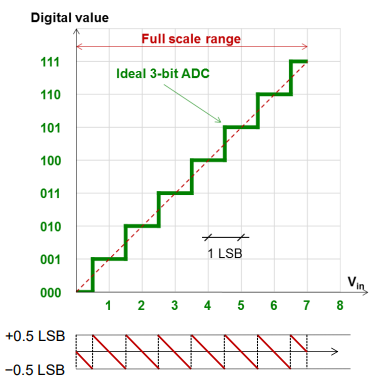
\includegraphics[width=0.85\linewidth]{quantizationerror.png}
\end{concept}



\begin{concept}{Gain Error}
\begin{itemize}
    \item Difference in slope between actual and ideal transfer function
    \item Expressed in LSB or as percentage of full-scale range (\%FSR)
    \item Can be corrected through calibration (HW/SW)
    \item Full-Scale Error = Offset Error + Gain Error
\end{itemize}

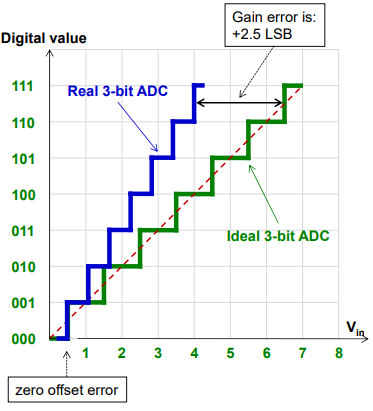
\includegraphics[width=0.8\linewidth]{gainerror.png}
\end{concept}

\begin{concept}{Offset Error} (Zero-scale error)
\begin{itemize}
    \item Deviation from ideal ADC at zero input
    \item For ideal ADC, first transition occurs at 0.5 LSB
    \item Can be corrected using microcontroller calibration
    \item Measuring: Zero-scale voltage is applied to analog input and increased until first digital transition occurs
\end{itemize}
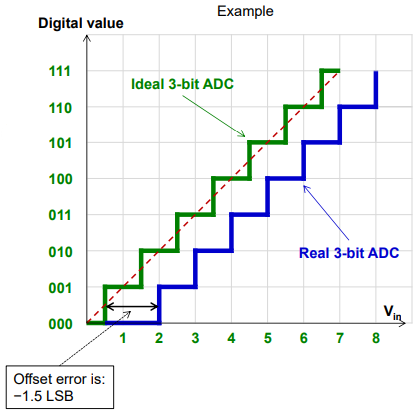
\includegraphics[width=0.85\linewidth]{offseterror.png}
\end{concept}

\begin{formula}{ADC Calculations}\\
\textbf{LSB Voltage}:
$$
V_{LSB} = \frac{V_{REF}}{2^N}
$$

\textbf{Digital Output Value}:
$$
D_{out} = \frac{V_{in} \times 2^N}{V_{REF}}
$$

\textbf{Analog Input from Digital Value}:
$$
V_{in} = \frac{D_{out} \times V_{REF}}{2^N}
$$

\textbf{FSR} (Full Scale Range):
$$FSR = V_{REF} - 1 LSB$$

\textbf{Percent Full Scale Range}:
$$
\%FSR = \frac{V_{in}}{V_{REF}} \times 100\%
$$
\end{formula}

\multend

\begin{KR}{Analyzing ADC Errors}
\paragraph{Understand error types}
\begin{itemize}
    \item \textbf{Quantization error:} Inherent error between -0.5 LSB and +0.5 LSB
    \item \textbf{Offset error:} Deviation from ideal transfer function at zero input
    \item \textbf{Gain error:} Deviation of the slope from ideal transfer function
    \item \textbf{Full-scale error:} Combination of offset and gain error at maximum input
\end{itemize}

\paragraph{Determine ADC resolution}
\begin{itemize}
    \item Calculate LSB size and FSR (Full Scale Range)
\end{itemize}

\paragraph{Draw ideal transfer function}
\begin{itemize}
    \item Plot digital output vs. analog input
    \item Idealer ADC: erste Transition bei 0.5 LSB, aach subsequent transition at (i + 0.5) × LSB
    \item For N-bit ADC: 2$^N$ - 1 total steps
\end{itemize}

\paragraph{Calculate error values}
\begin{itemize}
    \item \textbf{Offset error in LSB:} Measure deviation at zero input
    \item \textbf{Offset error in volts:} Multiply LSB by offset error in LSB
    \item \textbf{Gain error in LSB:} Difference between actual and ideal slope
    \item \textbf{Error as percentage of FSR (\%FSR):} (Error in volts / FSR in volts) × 100\%
\end{itemize}

\paragraph{Transfer-Funktion zeichnen}
    \begin{enumerate}
        \item Verschiebe ideale Funktion um Offset-Fehler (positiv = rechts, negativ = links)
        \item Erste Transition: 0.5 LSB + Offset\_Error
    \end{enumerate}
\end{KR}

\begin{example2}{3-Bit ADC mit Offset-Fehler}
    Idealer 3-Bit ADC mit V\_REF = 2V, Offset-Fehler = -1.5 LSB
    
    \tcblower

    \begin{minipage}{0.5\linewidth}
    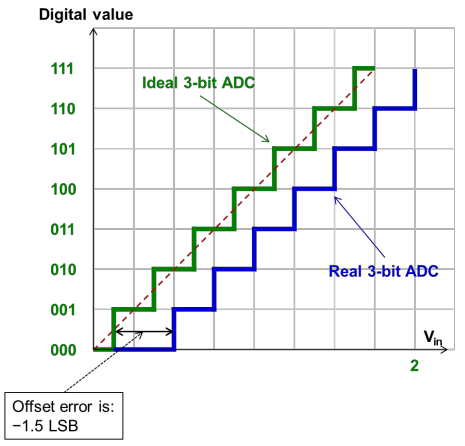
\includegraphics[width=0.8\linewidth]{adc_offset_ex.png}
    \end{minipage}
    \begin{minipage}{0.5\linewidth}
        In case of a positive offset error of +1.5 LSB, the graph will look like this:\\
        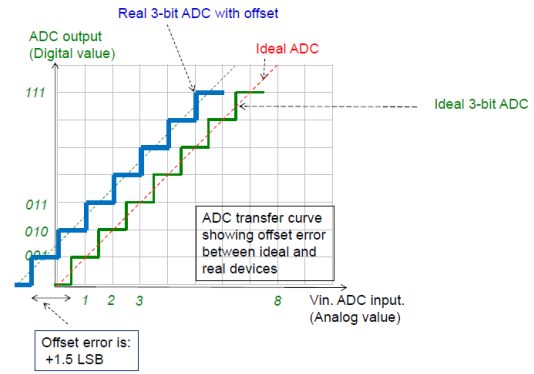
\includegraphics[width=\linewidth]{adc_positive_offset.png}
    \end{minipage}

    1. \textbf{Ideal transfer function:}
    \begin{itemize}
        \item N = 3 bits → 8 possible output codes (000 to 111)
        \item LSB = 2V / $2^3$ = 2V / 8 = 0.25V
        \item First transition: 0.5 × LSB = 0.125V
        \item Code transitions at: 0.125V, 0.375V, 0.625V, 0.875V, 1.125V, 1.375V, 1.625V
    \end{itemize}

    2. \textbf{Actual transfer function with offset error:}
    \begin{itemize}
        \item Offset error = -1.5 LSB (entire transfer function shifts left)
        \item Offset Error in volts: all transitions shift by -1.5 × 0.25V = -0.375V (Offset error $\times$ LSB)
        \item New transitions at: -0.25V, 0V, 0.25V, 0.5V, 0.75V, 1V, 1.25V
        \item Full Scale Range (FSR) = 2V - 0.25V = 1.75V
        \item Offset-Fehler (\%FSR) = 0.375V $\times$ 100 / 1.75V = 21.43\%
    \end{itemize}

    
    \textbf{3. Zusammenfassung:}
    \begin{itemize}
        \item Ideale erste Transition: 0.5 LSB = 0.125V
        \item Reale erste Transition: 0.125V - 0.375V = -0.25V
        \item Gesamte Kurve um 1.5 LSB nach links verschoben
    \end{itemize}
    
    \textbf{Digitale Werte:}
    Real-ADC erreicht digitalen Wert 001 bereits bei negativer Eingangsspannung, während ideal-ADC erst bei 0.125V den Wert 001 erreichen würde.
\end{example2}



\subsubsection{ADC on STM32F4}

\begin{concept}{STM32F4 ADC Architecture}\\
The STM32F4 includes ADC modules with the following features:
\begin{itemize}
    \item Three ADCs (ADC1, ADC2, ADC3)
    \item 12-bit resolution (configurable to 10, 8, or 6 bits)
    \item Up to 24 external channels (16 on each ADC)
    \item Internal channels: \\ temperature sensor, V$_{REFINT}$, V$_{BAT}$
\end{itemize}
 Multiple operating modes:
    \begin{itemize}
        \item Single conversion vs. continuous conversion
        \item Single channel vs. scan mode (multiple channels)
    \end{itemize}
Sampling and conversion features:
\begin{itemize}
    \item Maximum sampling rate up to 2.4 MSPS (million samples per second)
    \item DMA capability and configurable sampling time
    \item Analog watchdog for threshold monitoring
\end{itemize}
\end{concept}


\begin{theorem}{Simplified ADC Diagram}\\
    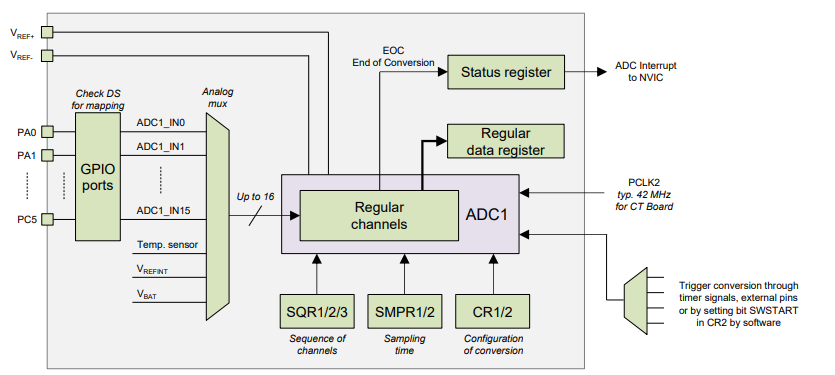
\includegraphics[width=\linewidth]{adcdiagram.png}
\end{theorem}


\subsubsection{ADC Modes and Conversion}

\begin{definition}{ADC Conversion Modes}\\
    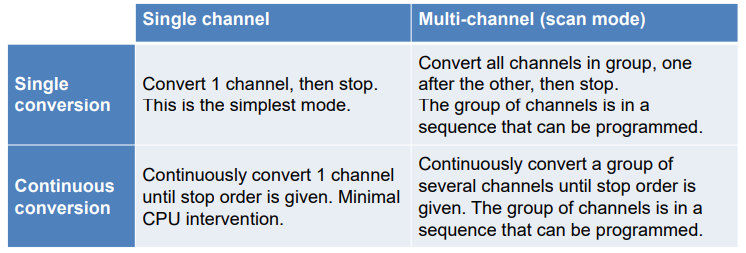
\includegraphics[width=0.8\linewidth]{adcconversionmodes.png}
\end{definition}





\begin{concept}{ADC Conversion Modes Comparison}\\
\textbf{Single vs. Continuous Conversion}:
\begin{itemize}
    \item \textbf{Single Conversion}: Performs one conversion, then stops
    \item \textbf{Continuous Conversion}: Continuously performs conversions without CPU intervention\\
    Minimal CPU intervention for setups $\rightarrow$ ADC doesn't require CPU intervention to start and beware overwriting results
\end{itemize}
\textbf{Single Channel vs. Scan Mode}:
\begin{itemize}
    \item \textbf{Single Channel}: Converts one channel only
    \item \textbf{Scan Mode}: Converts multiple channels in sequence
\end{itemize}
This results in four possible combinations:
\begin{itemize}
    \item Single channel, single conversion (simplest mode)
    \item Single channel, continuous conversion (monitor one input)
    \item Multi-channel, single conversion (read multiple inputs once)
    \item Multi-channel, continuous conversion (monitor multiple inputs)
\end{itemize}

\end{concept}

\subsubsection{ADC Timing}

\begin{KR}{ADC Timing Diagramm}\\
    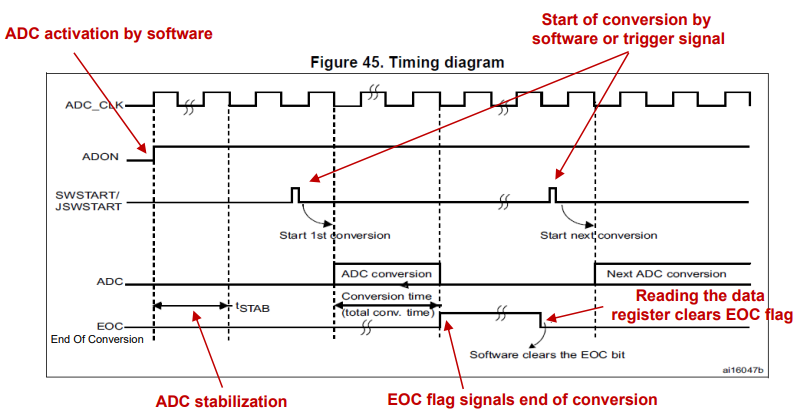
\includegraphics[width=0.8\linewidth]{adc_timing_diagram.png}
\end{KR}

\begin{concept}{ADC Timing}\\
    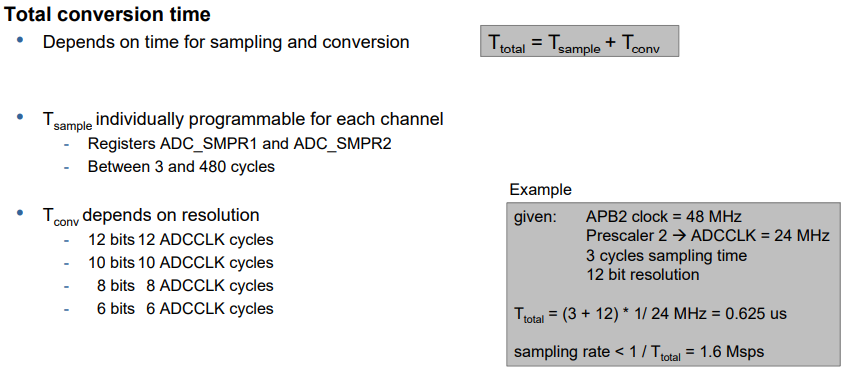
\includegraphics[width=\linewidth]{adctiming.png}
\end{concept}




\raggedcolumns
\columnbreak

\subsection{Programming the ADC - STM32F4}

\begin{definition}{Functional summary of ADC}\\
    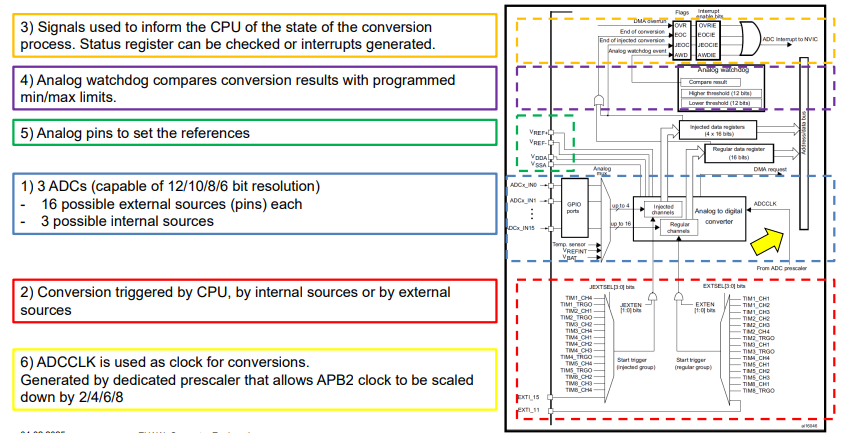
\includegraphics[width=\linewidth]{adcsummary.png}
\end{definition}

\begin{definition}{ADC Registers}\\
Key ADC registers on STM32F4:
\begin{itemize}
    \item \textbf{ADC\_SR}: Status register (flags for EOC, overrun, etc.)
    \item \textbf{ADC\_CR1}: Control register 1 (scan mode, resolution, etc.)
    \item \textbf{ADC\_CR2}: Control register 2 (conversion start, data alignment, etc.)
    \item \textbf{ADC\_SMPRx}: Sample time registers
    \item \textbf{ADC\_SQRx}: Regular sequence registers
    \item \textbf{ADC\_DR}: Data register (conversion result)
    \item \textbf{ADC\_CCR}: Common control register (for all ADCs)
\end{itemize}
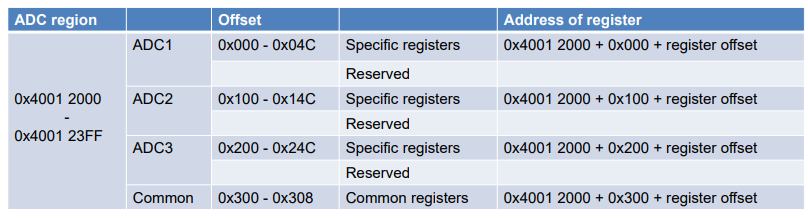
\includegraphics[width=\linewidth]{adcregisters1.png}\\
\important{SEP Handout Beilage ADC: addresses and configurations for ADC registers, Data Alignment}
\end{definition}

\begin{concept}{ADC Common Registers}\\
    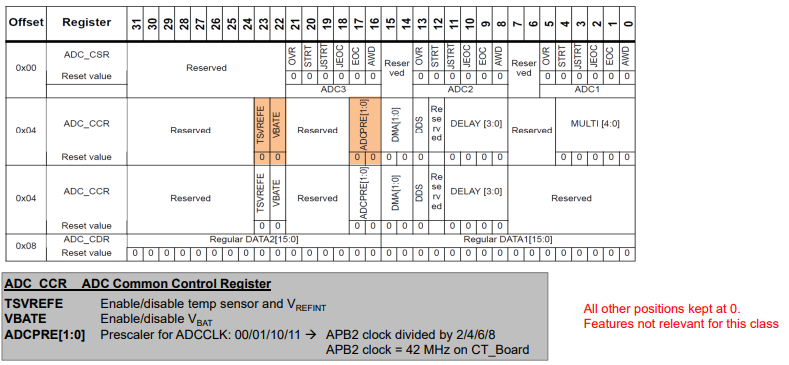
\includegraphics[width=\linewidth]{adccommonregisters.png}
\end{concept}

\begin{concept}{Specific Registers for each ADC}\\
    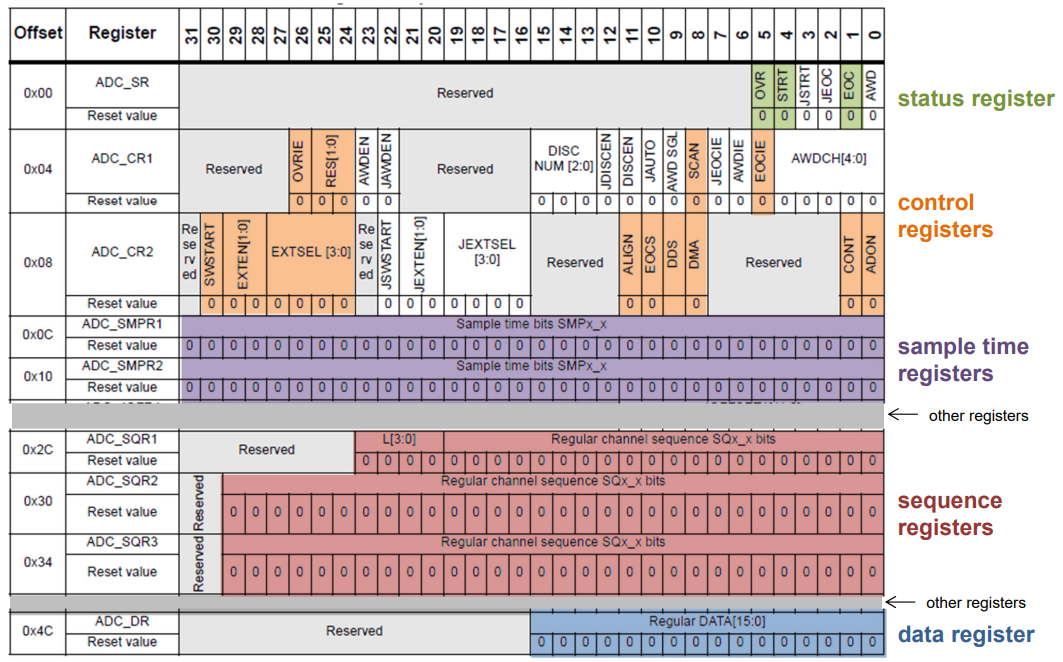
\includegraphics[width=\linewidth]{sepcificregistersadc.png}
\end{concept}

\begin{theorem}{ADC Register Bits}\\
    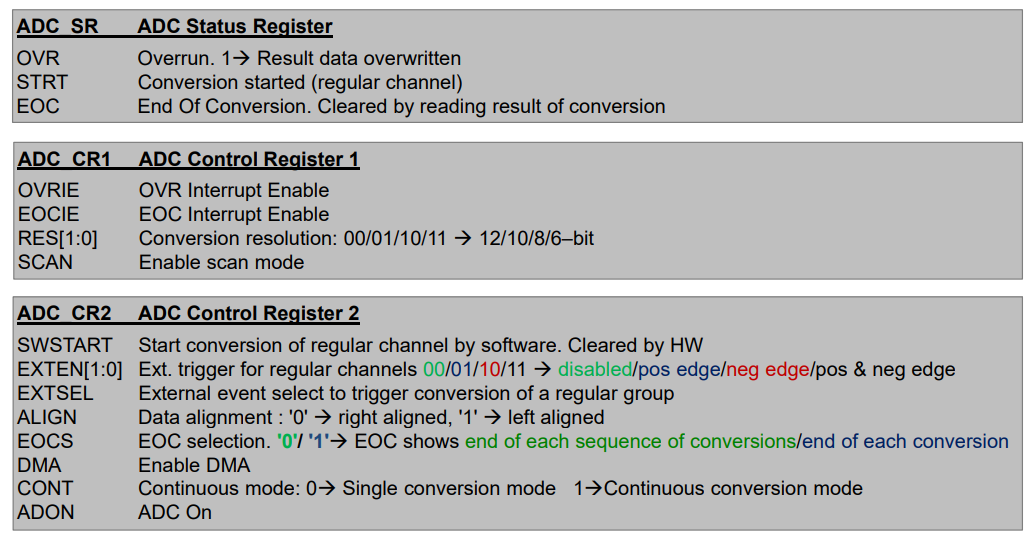
\includegraphics[width=\linewidth]{adcregisterbits.png}
\end{theorem}

\begin{corollary}{Sampling Time Registers}\\
    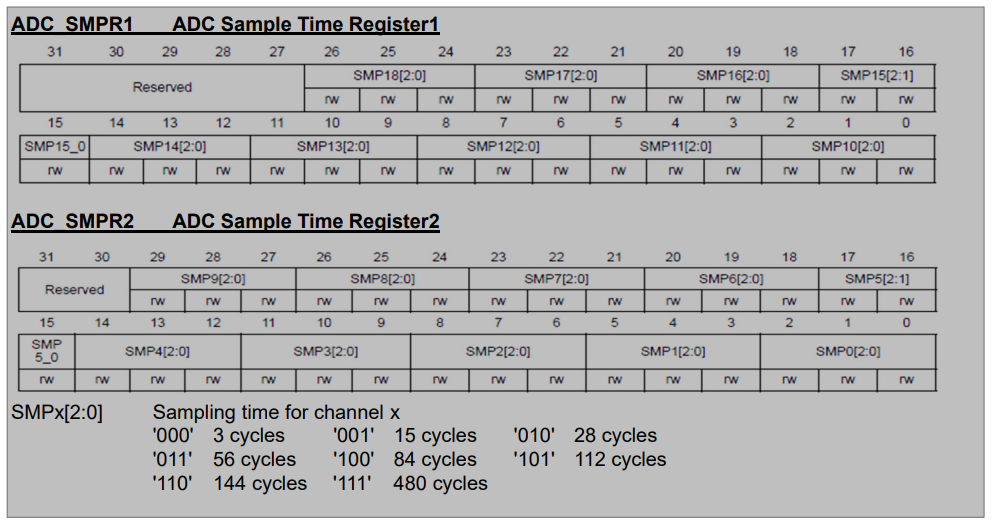
\includegraphics[width=\linewidth]{samplingtimeregistersadc.png}    
\end{corollary}

\begin{corollary}{Sequence Registers}\\
    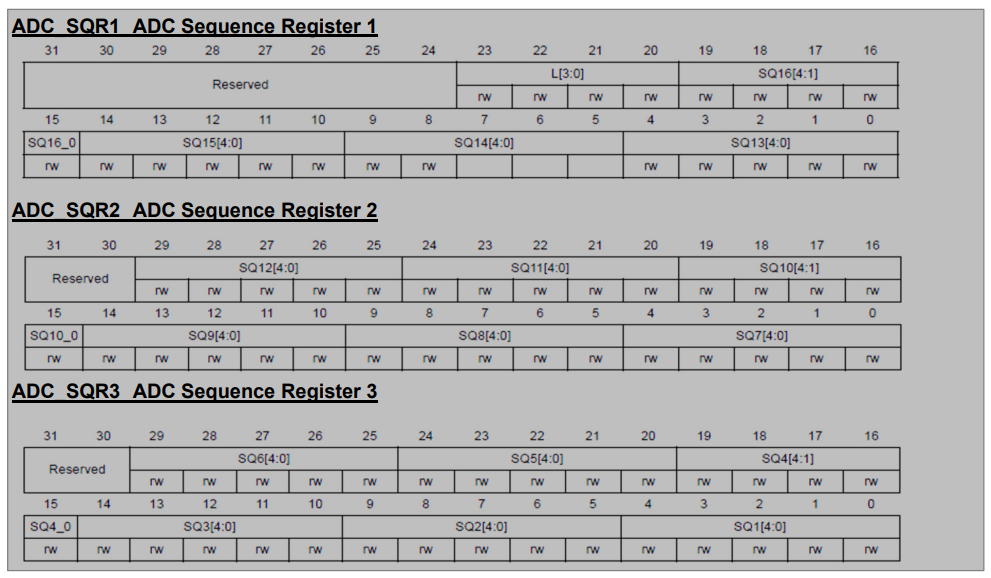
\includegraphics[width=\linewidth]{sequenceadcregisters.png}\\
    Sequence of channels:\\
    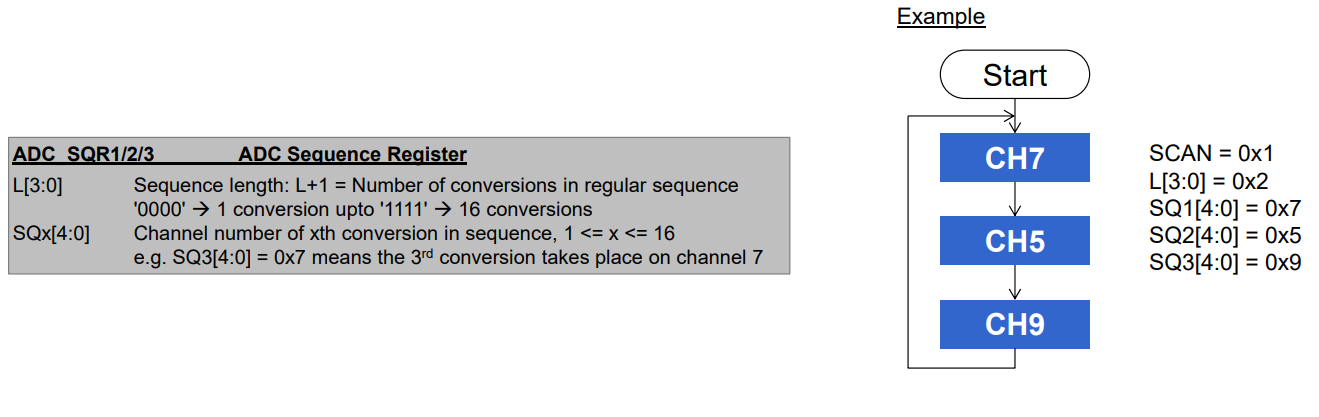
\includegraphics[width=\linewidth]{sequenceofchannelsadc.png}
\end{corollary}

\begin{concept}{ADC-Register programmieren}
    \paragraph{Status-Register auswerten}
    \begin{itemize}
        \item EOC (End of Conversion): Bit 1 in ADC\_SR
        \item OVR (Overrun): Bit 5 in ADC\_SR
        \item Warten auf Conversion: \texttt{while (!(ADC\_SR \& 0x02))}
        \item Overrun prüfen: \texttt{if (ADC\_SR \& 0x20)}
    \end{itemize}
    
    \paragraph{Auflösung konfigurieren}
    \begin{itemize}
        \item RES[1:0] in ADC\_CR1 Register (Bits 25:24)
        \item 00: 12-bit, 01: 10-bit, 10: 8-bit, 11: 6-bit
        \item Einzelne Bits setzen/löschen mit Bit-Masken
    \end{itemize}
    
    \paragraph{Adressen berechnen}
    \begin{itemize}
        \item ADC1: 0x40012000 + Register\_Offset
        \item ADC2: 0x40012100 + Register\_Offset  
        \item ADC3: 0x40012200 + Register\_Offset
        \item Siehe Reference Manual für genaue Offsets
    \end{itemize}
    
    \paragraph{Bit-Manipulation}
    \begin{itemize}
        \item Bit setzen: \texttt{REG |= (1 << bit\_nr)}
        \item Bit löschen: \texttt{REG \&= \~{}(1 << bit\_nr)}
        \item Mehrere Bits: erst löschen, dann setzen
    \end{itemize}
\end{concept}
\begin{remark}
    Bei ADC-Registern ist es wichtig, die korrekten Bit-Positionen zu verwenden. EOC ist Bit 1 (nicht Bit 0), OVR ist Bit 5. Die Auflösung wird durch zwei Bits (RES[1:0]) in Bits 25:24 des CR1-Registers gesteuert.
\end{remark}

\begin{concept}{Performing ADC Conversion}
\paragraph{Start conversion}
Trigger the conversion using software or external trigger.
\paragraph{Wait for completion}
Check the EOC flag to determine when conversion is complete.
\paragraph{Read result}
Read the data register to get the conversion result.

\begin{lstlisting}[language=C, style=basesmol]
// Function to perform single ADC conversion
uint16_t ADC_ReadChannel(void) {
    // Start conversion
    ADC1->CR2 |= ADC_CR2_SWSTART;  // Software trigger to start conversion
    
    // Wait for conversion to complete
    while (!(ADC1->SR & ADC_SR_EOC)) { }
    
    // Read and return result
    return ADC1->DR;
}

// Function to convert ADC value to voltage
float ADC_ConvertToVoltage(uint16_t adcValue) {
    // Assuming VREF = 3.3V and 12-bit resolution (4096 levels)
    float voltage = (float)adcValue * 3.3f / 4095.0f;
    return voltage;
}
\end{lstlisting}
\end{concept}

\begin{KR}{Configuring and Using STM32 ADCs}
\paragraph{Enable peripheral clocks}
\begin{itemize}
    \item Enable GPIO clock for analog pin
    \item Enable ADC clock in RCC register
\end{itemize}

\paragraph{Configure GPIO pin for analog mode}
\begin{itemize}
    \item Set GPIO MODE register bits to analog mode (11)
\end{itemize}

\paragraph{Configure ADC common settings}
\begin{itemize}
    \item Configure ADC clock prescaler in ADC\_CCR
    \item Enable/disable temperature sensor and internal reference
\end{itemize}

\paragraph{Configure ADC specific settings}
\begin{itemize}
    \item Set resolution in ADC\_CR1 (RES bits)
    \item Configure scan mode if using multiple channels
    \item Set conversion mode in ADC\_CR2 (CONT bit):
    \begin{itemize}
        \item 0: Single conversion
        \item 1: Continuous conversion
    \end{itemize}
    \item Set data alignment in ADC\_CR2 (ALIGN bit)
    \item Configure ADC trigger source if needed
\end{itemize}

\paragraph{Configure channel settings}
\begin{itemize}
    \item Set sampling time in ADC\_SMPR1/2 registers
    \item Configure regular sequence in ADC\_SQR1/2/3:
    \begin{itemize}
        \item Set sequence length in L[3:0] bits
        \item Set channel order in SQx[4:0] bits
    \end{itemize}
\end{itemize}

\paragraph{Start conversion and read results}
\begin{itemize}
    \item Enable ADC by setting ADON bit in ADC\_CR2
    \item Start conversion by setting SWSTART bit in ADC\_CR2
    \item Poll EOC flag in ADC\_SR or use interrupt
    \item Read conversion result from ADC\_DR
\end{itemize}

\begin{lstlisting}[language=C, style=basesmol]
// Example: Configure ADC1 Channel 0 (PA0) for single conversion
// Step 1: Enable GPIO and ADC clocks
RCC->AHB1ENR |= RCC_AHB1ENR_GPIOAEN;  // Enable GPIOA clock
RCC->APB2ENR |= RCC_APB2ENR_ADC1EN;   // Enable ADC1 clock
// Step 2: Configure PA0 as analog input
GPIOA->MODER |= GPIO_MODER_MODER0;  // Analog mode (0b11)
// Step 3: Configure ADC parameters
// ADC Common Control Register
ADC->CCR &= ~ADC_CCR_ADCPRE;  // ADCPRE = 0 (APB2/2, typically 42MHz/2 = 21MHz)
// ADC1 Control Register 1
ADC1->CR1 &= ~ADC_CR1_RES;    // 12-bit resolution (default)
ADC1->CR1 &= ~ADC_CR1_SCAN;   // Disable scan mode (single channel)
// ADC1 Control Register 2
ADC1->CR2 &= ~ADC_CR2_CONT;   // Single conversion mode
ADC1->CR2 &= ~ADC_CR2_ALIGN;  // Right alignment
ADC1->CR2 &= ~ADC_CR2_EXTEN;  // Software trigger
// Step 4: Configure channel and sampling time
// Configure for channel 0
ADC1->SQR1 &= ~ADC_SQR1_L;     // 1 conversion in regular sequence
ADC1->SQR3 &= ~ADC_SQR3_SQ1;   // Clear channel selection
ADC1->SQR3 |= (0 << ADC_SQR3_SQ1_Pos);  // Channel 0 as first conversion
// Set sampling time for channel 0 (e.g., 84 cycles)
ADC1->SMPR2 &= ~ADC_SMPR2_SMP0;  // Clear bits
ADC1->SMPR2 |= (4 << ADC_SMPR2_SMP0_Pos);  // 84 cycles
// Step 5: Enable ADC
ADC1->CR2 |= ADC_CR2_ADON;  // Turn on ADC
\end{lstlisting}
\end{KR}







\begin{example2}{ADC Configuration and Usage Example}
Write C code to configure and use ADC1 to read from channel 5 with 12-bit resolution in single conversion mode. The code should:

\begin{enumerate}
    \item Wait until ADC1 conversion has completed
    \item Set an 8-bit variable (var2) to 0xFF if there was a loss of data on ADC2, otherwise reset that variable to 0
    \item Set ADC3 resolution to 10-bit
\end{enumerate}

Use register addresses from the provided documentation.

\paragraph{Solution:}
First, let's define the relevant register addresses:
\begin{lstlisting}[language=C, style=basesmol]
// ADC1 registers
#define ADC1_SR     (*((volatile uint32_t*)(0x40012000)))  // Status register
#define ADC1_CR1    (*((volatile uint32_t*)(0x40012004)))  // Control register 1
#define ADC1_CR2    (*((volatile uint32_t*)(0x40012008)))  // Control register 2
#define ADC1_DR     (*((volatile uint32_t*)(0x4001204C)))  // Data register
// ADC2 registers
#define ADC2_SR     (*((volatile uint32_t*)(0x40012100)))  // Status register
// ADC3 registers
#define ADC3_CR1    (*((volatile uint32_t*)(0x40012204)))  // Control register 1
// Bit positions
#define ADC_SR_EOC  (1 << 1)  // End of conversion flag
#define ADC_SR_OVR  (1 << 5)  // Overrun flag
#define ADC_CR1_RES_MASK (3 << 24)  // Resolution mask
#define ADC_CR1_RES_10BIT (1 << 24)  // 10-bit resolution
\end{lstlisting}

Now, let's solve each part of the problem:

1. \textbf{Wait until ADC1 conversion has completed} $\rightarrow$ wait for the EOC flag in ADC1\_SR (Bit 1)
\begin{lstlisting}[language=C, style=basesmol]
// Wait for end of conversion flag
while (!(ADC1_SR & ADC_SR_EOC)) {
    // Empty loop, wait until EOC is set
}
\end{lstlisting}

2. \textbf{Check for overrun on ADC2 and set var2 accordingly} $\rightarrow$ check the OVR flag in ADC2\_SR (Bit 5)
\begin{lstlisting}[language=C, style=basesmol]
uint8_t var2;
if (ADC2_SR & ADC_SR_OVR) {
    var2 = 0xFF;  // Overrun occurred
} else {
    var2 = 0x00;  // No overrun
}
\end{lstlisting}

3. \textbf{Set ADC3 resolution to 10-bit} $\rightarrow$ clear the RES bits in ADC3\_CR1 and set to 10-bit
\begin{lstlisting}[language=C, style=basesmol]
ADC3_CR1 &= ~ADC_CR1_RES_MASK;  // Clear bits
ADC3_CR1 |= ADC_CR1_RES_10BIT;  // Set 10-bit resolution
\end{lstlisting}
\end{example2}

\begin{example2}{ADC Configuration Exercise}\\
Configure ADC1 to measure an analog voltage on pin PA5, with 12-bit resolution. Convert the result to a voltage between 0-3.3V.
\tcblower
1. Configure PA5 as an analog input\\
2. Configure ADC1 for 12-bit resolution, single conversion, single channel\\
3. Set appropriate sampling time\\
4. Perform conversion and convert result to voltage

\begin{lstlisting}[language=C, style=basesmol]
// Configure PA5 as analog input
RCC->AHB1ENR |= RCC_AHB1ENR_GPIOAEN;  // Enable GPIOA clock
RCC->APB2ENR |= RCC_PB2ENR_ADC1EN;   // Enable ADC1 clock
GPIOA->MODER |= GPIO_MODER_MODER5;    // Set PA5 to analog mode (0b11)

// Configure ADC1
ADC1->CR1 &= ~ADC_CR1_RES;     // 12-bit resolution (default)
ADC1->CR2 &= ~ADC_CR2_CONT;    // Single conversion mode
ADC1->CR2 &= ~ADC_CR2_ALIGN;   // Right alignment

// Configure for channel 5 (PA5)
ADC1->SQR1 &= ~ADC_SQR1_L;      // 1 conversion in sequence
ADC1->SQR3 &= ~ADC_SQR3_SQ1;    // Clear channel selection
ADC1->SQR3 |= (5 << ADC_SQR3_SQ1_Pos);  // Channel 5 as first conversion

// Set sampling time (84 cycles)
ADC1->SMPR2 &= ~ADC_SMPR2_SMP5;
ADC1->SMPR2 |= (4 << ADC_SMPR2_SMP5_Pos);

// Enable ADC
ADC1->CR2 |= ADC_CR2_ADON;

// Function to read ADC and convert to voltage
float ReadVoltage(void) {
    // Start conversion
    ADC1->CR2 |= ADC_CR2_SWSTART;
    
    // Wait for conversion to complete
    while (!(ADC1->SR & ADC_SR_EOC)) { }
    
    // Read ADC value
    uint16_t adcValue = ADC1->DR;
    
    // Convert to voltage (0-3.3V)
    float voltage = (float)adcValue * 3.3f / 4095.0f;
    
    return voltage;
}
\end{lstlisting}
\end{example2}



\begin{KR}{Multi-Channel ADC Configuration}
\paragraph{Configure scan mode}
Enable scan mode to convert multiple channels.
\paragraph{Set up channel sequence}
Configure the sequence and number of channels.
\paragraph{Process results}
Read results for each channel in sequence.

\begin{lstlisting}[language=C, style=basesmol]
// Configure ADC for multi-channel scanning (channels 0, 1, and 4)

// Enable scan mode
ADC1->CR1 |= ADC_CR1_SCAN;

// Set number of conversions in sequence (3)
ADC1->SQR1 &= ~ADC_SQR1_L;
ADC1->SQR1 |= (2 << ADC_SQR1_L_Pos);  // L = 2 means 3 conversions

// Set channel sequence
ADC1->SQR3 = 0;  // Clear all
ADC1->SQR3 |= (0 << ADC_SQR3_SQ1_Pos);  // CH0 as 1st conversion
ADC1->SQR3 |= (1 << ADC_SQR3_SQ2_Pos);  // CH1 as 2nd conversion
ADC1->SQR3 |= (4 << ADC_SQR3_SQ3_Pos);  // CH4 as 3rd conversion

// Set sampling times for each channel
ADC1->SMPR2 &= ~(ADC_SMPR2_SMP0 | ADC_SMPR2_SMP1 | ADC_SMPR2_SMP4);
ADC1->SMPR2 |= (4 << ADC_SMPR2_SMP0_Pos);  // 84 cycles for CH0
ADC1->SMPR2 |= (4 << ADC_SMPR2_SMP1_Pos);  // 84 cycles for CH1
ADC1->SMPR2 |= (4 << ADC_SMPR2_SMP4_Pos);  // 84 cycles for CH4
\end{lstlisting}
\end{KR}

\begin{example2}{Programming ADC} Example for PF8\\
    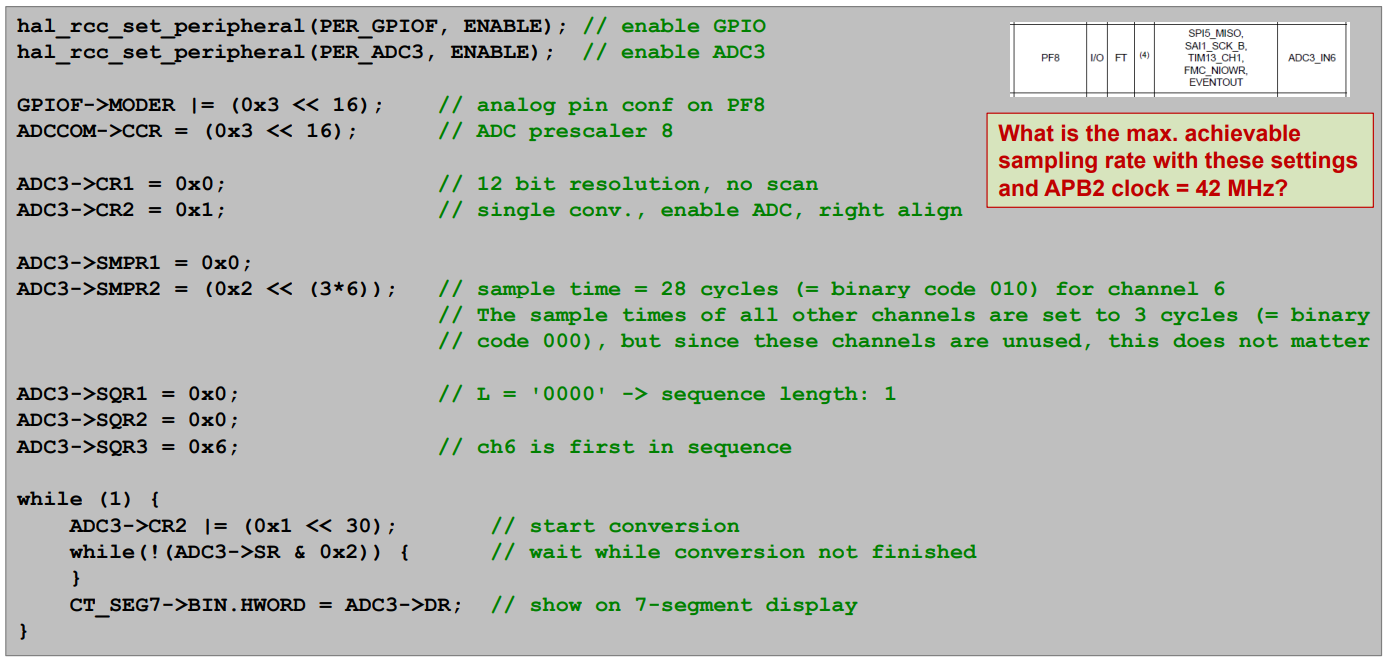
\includegraphics[width=\linewidth]{adcprogrammingexample.png}
\end{example2}



\raggedcolumns
\columnbreak

\subsection{DAC (Digital-to-Analog Converter)}
\begin{definition}{DAC Overview}\\
    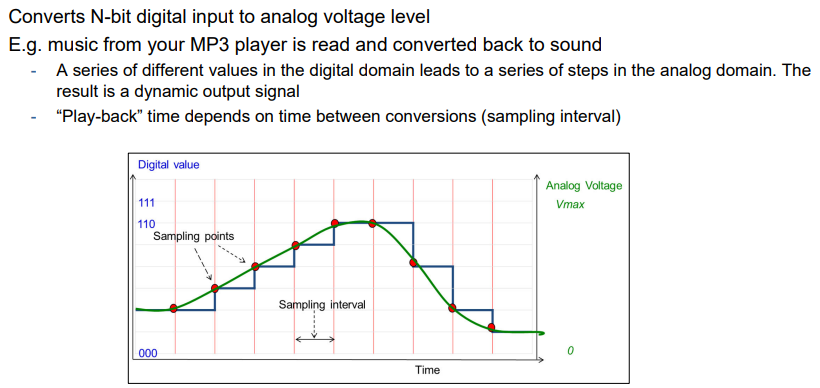
\includegraphics[width=0.8\linewidth]{dacoverview.png}
\end{definition}

\begin{concept}{DAC Characteristics}\\
    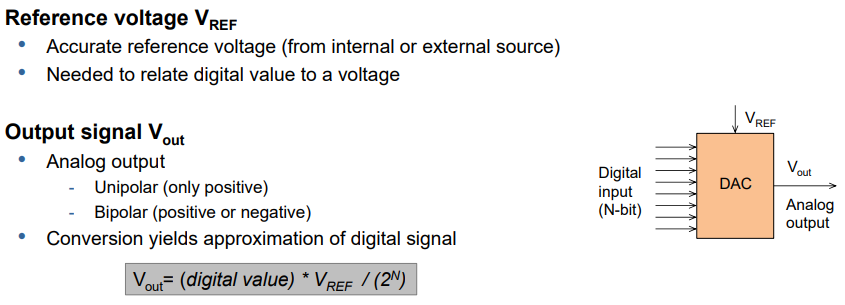
\includegraphics[width=0.8\linewidth]{dac_characteristics.png}
\end{concept}

\begin{theorem}{Example Flash DAC}\\
    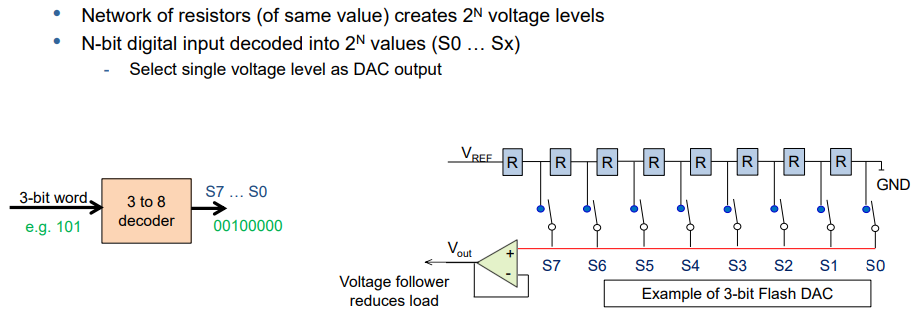
\includegraphics[width=\linewidth]{flashdac.png}
\end{theorem}


